\documentclass[border=8pt]{standalone}
\usepackage{amsmath}
\usepackage{amssymb}
\usepackage[normalem]{ulem}
\usepackage{tikz}
\usetikzlibrary{arrows.meta,calc,decorations.pathreplacing,patterns,shapes.geometric,positioning,shadings}

\begin{document}
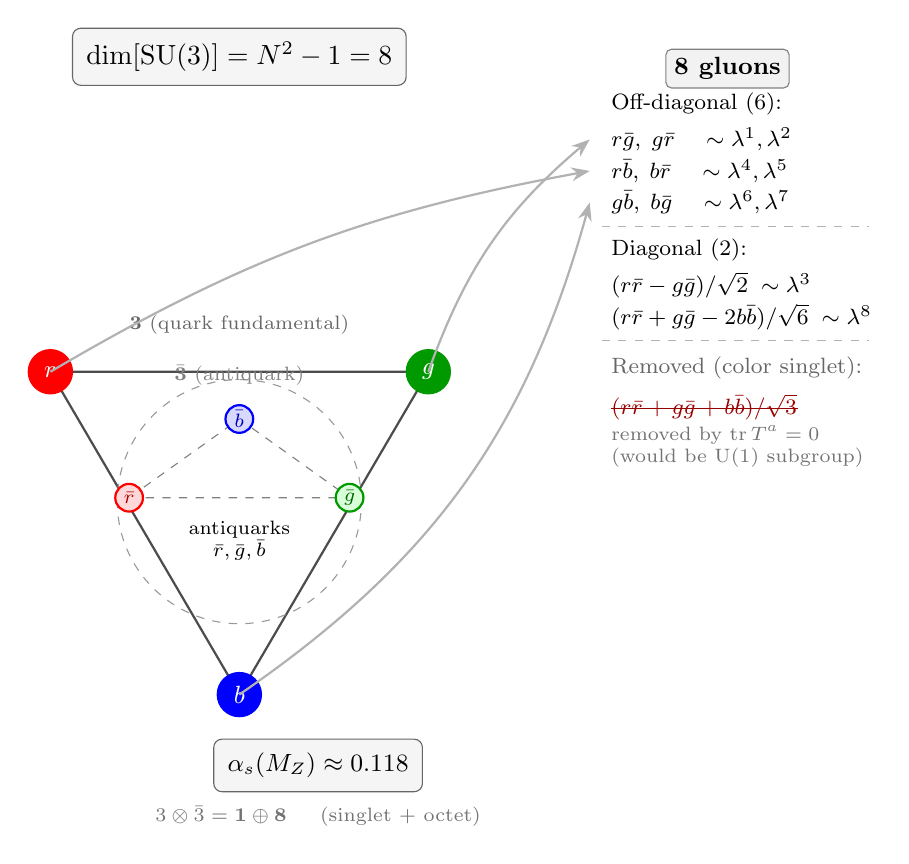
\begin{tikzpicture}[>=Stealth,font=\sffamily]

% ===== Top dimension formula =====
\node[draw=black!60,rounded corners=3pt,fill=gray!8,inner sep=5pt] (dimbox)
    at (0,5.6) {$\dim[\mathrm{SU}(3)]=N^{2}-1=8$};

% ===== Color triangle (quark fundamental) =====
% Equilateral triangle vertices
\coordinate (R) at (-2.4,1.6);
\coordinate (G) at ( 2.4,1.6);
\coordinate (B) at ( 0.0,-2.5);

% Triangle edges
\draw[thick,black!70] (R) -- (G) -- (B) -- cycle;

% Inverted dashed triangle for antiquarks
\coordinate (Rb) at (-1.4, 0.0);
\coordinate (Gb) at ( 1.4, 0.0);
\coordinate (Bb) at ( 0.0, 1.0);
\draw[dashed,black!50] (Rb) -- (Gb) -- (Bb) -- cycle;

% Center circle
\draw[dashed,black!40] (0,-0.05) circle (1.55);
\node[font=\scriptsize,align=center] at (0,-0.55) {antiquarks\\$\bar r,\bar g,\bar b$};

% Quark color dots
\filldraw[red]   (R) circle (8pt) node[white,font=\bfseries\small] {$r$};
\filldraw[green!60!black] (G) circle (8pt) node[white,font=\bfseries\small] {$g$};
\filldraw[blue]  (B) circle (8pt) node[white,font=\bfseries\small] {$b$};

% Antiquark dots (smaller, ringed)
\draw[red,  thick,fill=red!15]   (Rb) circle (5pt) node[red!70!black,font=\scriptsize] {$\bar r$};
\draw[green!60!black,thick,fill=green!15] (Gb) circle (5pt) node[green!40!black,font=\scriptsize] {$\bar g$};
\draw[blue, thick,fill=blue!15]  (Bb) circle (5pt) node[blue!70!black,font=\scriptsize] {$\bar b$};

% Triangle label
\node[font=\scriptsize,black!60] at (0,2.2) {$\mathbf{3}$ (quark fundamental)};
\node[font=\scriptsize,black!50] at (0, 1.55) {$\bar{\mathbf{3}}$ (antiquark)};

% ===== Right column: 8 gluons =====
\def\xL{4.6}
\def\yT{5.0}

\node[draw=black!50,fill=black!5,rounded corners=2pt,inner sep=3pt,font=\small\bfseries]
    at (\xL+1.6,\yT+0.45) {8 gluons};

% Group 1: 6 off-diagonal
\node[font=\footnotesize,anchor=west] at (\xL,\yT) {Off-diagonal (6):};
\node[font=\footnotesize,anchor=west] at (\xL,\yT-0.45) {$r\bar g,\; g\bar r$ \quad $\sim\lambda^{1},\lambda^{2}$};
\node[font=\footnotesize,anchor=west] at (\xL,\yT-0.85) {$r\bar b,\; b\bar r$ \quad $\sim\lambda^{4},\lambda^{5}$};
\node[font=\footnotesize,anchor=west] at (\xL,\yT-1.25) {$g\bar b,\; b\bar g$ \quad $\sim\lambda^{6},\lambda^{7}$};

% Separator
\draw[black!30,dashed] (\xL,\yT-1.55) -- (\xL+3.4,\yT-1.55);

% Group 2: 2 diagonal
\node[font=\footnotesize,anchor=west] at (\xL,\yT-1.85) {Diagonal (2):};
\node[font=\footnotesize,anchor=west] at (\xL,\yT-2.30) {$(r\bar r-g\bar g)/\sqrt{2}\;\sim\lambda^{3}$};
\node[font=\footnotesize,anchor=west] at (\xL,\yT-2.70) {$(r\bar r+g\bar g-2 b\bar b)/\sqrt{6}\;\sim\lambda^{8}$};

% Separator
\draw[black!30,dashed] (\xL,\yT-3.00) -- (\xL+3.4,\yT-3.00);

% Removed: singlet
\node[font=\footnotesize,anchor=west,black!60] at (\xL,\yT-3.35) {Removed (color singlet):};
\node[font=\footnotesize,anchor=west,red!60!black] at (\xL,\yT-3.85)
    {\sout{$(r\bar r+g\bar g+b\bar b)/\sqrt{3}$}};
\node[font=\scriptsize,anchor=west,black!55,align=left] at (\xL,\yT-4.35)
    {removed by $\mathrm{tr}\,T^{a}=0$\\(would be U(1) subgroup)};

% Connecting arrows from triangle to gluon list
\draw[->,gray!60,thick] (G) to[bend left=15] (\xL-0.15,\yT-0.45);
\draw[->,gray!60,thick] (R) to[bend left=10] (\xL-0.15,\yT-0.85);
\draw[->,gray!60,thick] (B) to[bend right=20] (\xL-0.15,\yT-1.25);

% ===== Bottom: coupling at MZ =====
\node[draw=black!60,rounded corners=3pt,fill=gray!8,inner sep=5pt,font=\small]
    at (1.0,-3.4) {$\alpha_{s}(M_{Z})\approx 0.118$};

\node[font=\scriptsize,black!55,align=center] at (1.0,-4.05)
    {$3\otimes\bar{3}=\mathbf{1}\oplus\mathbf{8}$ \;\;\; (singlet $+$ octet)};

\end{tikzpicture}
\end{document}
